% !TeX spellcheck = en_US
%===================================== CHAP 3 =================================

\chapter{Basic Theory} \label{ch:Basic Theory}

Common to all the attack vectors described in Section \ref{sec:attack_vectors} is that the attacker rely on background knowledge, often also called auxiliary information, to perform their linkage attacks. Protecting a database against this threat has long been a major challenge in database design. Already back in 1977 Tore Dalenius \citep{dalenius1977towards} defined a desideratum for data privacy which says that: \begin{quote}
	Access to the published data should not enable the adversary to learn anything extra about target victim compared to no access to the database, even with the presence of any adversary’s background knowledge obtained from other sources.
\end{quote} 

This privacy goal was rejected by Cynthia Dwork, who showed the general impossibility of Dalenius' goal due to the existence of auxiliary information. Instead she chose to formulate a probabilistic privacy goal, which places an upper bound on how much the risk of privacy breach can increase by participating in a database.

%In a world where massive amounts of sensitive personal data are being collected, attacks on the individual's privacy are becoming more and more of a threat. One type of attack is the identification of an individual's personal information from massive data sets, such as people's movie ratings from the Netflix data set\cite{narayanan2008robust}, and the medical records of a former governor of Massachusetts\cite{barth2012re}. These types of privacy breaches may lead to the unwanted discovery of a person's embarrassing information, and could also lead to the theft of an individual's private data or identity.  
%
%Many different approaches have been tried by data custodians to privatize the data they hold, such as removing any columns containing Personally Identifiable Information (PII), anonymizing the data by providing k-anonymity protection\cite{sweeney2002k}, or perform group based anonymization through l-diversity\cite{machanavajjhala2007diversity}. All of these methods mentioned have been proved to be susceptible in some way or form to attacks \cite{ganta2008composition}. Motivated by these shortcomings, a researcher at Microsoft came up with a data theoretical framework called differential privacy, which operates off a solid mathematical foundation and have strong theoretical guarantees on the privacy and utility of the released data.

\section{Differential Privacy}
\label{section:differential_privacy}
The term "differential privacy" was defined by Dwork as a description of a promise, made by a data holder to a data subject: "You will not be affected, adversely or otherwise, by allowing your data to be used in any study or analysis, no matter what other studies, data sets, or information sources, are available." \citep{dwork2013algorithmic}
In an ideal situation, databases which implement differential privacy mechanisms can make confidential data widely available for accurate data analysis, without resorting to data usage agreements, data protection plans, or restricted views. Nevertheless, the Fundamental Law of Information Recovery states that overly accurate answers to too many questions will destroy privacy in a spectacular way \citep{dwork2013algorithmic}, meaning that data utility will eventually be consumed.

\subsection{Definition of Differential Privacy}
The classic example for explaining a security breach is the case of Mr White: Suppose you have access to a database that allows you to compute the income of all residents in a specified area. If you knew that Mr White was going to move, simply querying the database before and after his relocation would allow you to deduce his income. 

\begin{definition} The distance of two data sets, $d(D_1, D_2)$, denotes the minimum number of sample changes that are required to change $D_1$ into $D_2$.
\end{definition}

Formally, differential privacy is defined as follows:
A randomized function $M$ gives $\epsilon$-differential privacy if for all data sets $D_1$ and $D_2$ where $d(D_1, D_2)=1$, and all $S\subseteq Range(M)$,
\begin{eqnarray} \label{DiffPrivDef}
 Pr[M(D_1)\in S]\leq \mathrm{e}^{(\epsilon)}\times Pr[M(D_2)\in S]
 \end{eqnarray}

That is, the presence or absence of a particular record should not affect the probability of any given output of $M(D)$ by more than some multiplicative factor. 

Informally, the presence or absence of a single record in a database should not have a noticeable impact on the output of any queries sent to it. Though the existence of the database itself might allow attackers to learn information about a person, opting out of the database will not significantly help reduce the risk of information disclosure. Conversely, participating in the database does not significantly increase the risk of disclosure either, thus fulfilling Dworks promise quoted in the beginning of Section \ref{section:differential_privacy}.

Privacy preserving data analysis platforms such as PINQ\citep{mcsherry2009PINQ}, Airavat\citep{roy2010airavat} and Fuzz\citep{Haeberlen2011fuzz} have all implemented features such as privacy budgeting and noise mechanisms to compute useful queries while fulfilling Equation \ref{DiffPrivDef}.

\subsection{Privacy Budget}
\label{section:privacy_budget}
The quotient $\frac{Pr[M(D_1)\in S]}{Pr[M(D_2)\in S]}$ measures the extent to which an attacker can ascertain the difference between the two data sets\citep{abowd2008protective}. \cite{Sarathy2011evaluating} calls this ratio the ''knowledge gain ratio''. Differential privacy requires that this ratio is limited to $e^\epsilon$. This is because as the ratio grows larger, an attacker can determine with greater probability that the query result was obtained from one data set over the other.

Privacy budgeting was introduced to limit the amount of information a data analyst can obtain about any individual with data records in the data set. The data analysis platform will track every query to ensure that both individual queries and aggregation queries do not exceed the given budget. This privacy standard forbids further queries to the database once the budget has been consumed. 

Defining and depleting a privacy budget is possible due to the sequential composition property of $\epsilon$-differentially private mechanisms, as shown by \cite{mcsherry2009PINQ}. Given $N$ mechanisms $M_i$ that offer $\frac{\epsilon}{N}$-differential privacy, applying each mechanism $M_i$ in sequence offers $\epsilon$-differentially privacy.

%When making a practical implementation, the $\epsilon$ value represents the privacy budget of the data set. The budget value is set by the data analyst, but as it was shown in \cite{Sarathy2011evaluating} that the attacker's knowlfa edge gain rises exponentially with the rising number of queries. Setting a high value for $\epsilon$ will have a measurable impact on data privacy. 


\subsection{Noise Mechanisms}
Given a target function $f$ to compute on a database $D$, it is necessary to design a randomized function $M$ which fulfills Equation \ref{DiffPrivDef} while yielding a useful approximation to the true $f$. This randomized function $M$ can be created by adding noise to the computation of $f$. There are many different mechanisms for applying this noise, but the two most common are the Laplace mechanism and the Exponential mechanism. 

\subsubsection{Laplace Mechanism}
The Laplace mechanism involves adding random noise which follows the Laplace statistical distribution. The Laplace distribution centered around zero has only one parameter, its scale $b$, and this is proportional to its standard deviation. 
\begin{eqnarray} \label{LaplaceDisDef}
Lap(x|b) = \frac{1}{2b} exp (-\frac{|x|}{b})
\end{eqnarray}
When using the Laplace mechanism it is necessary to choose a suitable value for the parameter $b$. Increasing values of $b$ results in increased noise variance. The scale of $b$ is naturally dependent on the privacy parameter $\epsilon$, and also on the effect the presence or absence of a single record can have on the output of function $f$. This risk is called the sensitivity of the function, and is defined mathematically as:
\begin{eqnarray} \label{eq:sensitivity_def}
\Delta f=\underset{D_1,D_2}{max}||\mathit{f(D_1)}-\mathit{f(D_2)}||_{1}
 \end{eqnarray}
 \missingfigure[figwidth=6cm]{Picture showing the laplacian distribution} \unsure{Not sure if we need the pic. Alex: I think we do.}]
%$
% <math>f(x|\mu,b) = \frac{1}{2b} \exp \left( -\frac{|x-\mu|}{b} \right) \,\!</math>
% <math> = \frac{1}{2b}
% \left\{\begin{matrix}
% 	\exp \left( -\frac{\mu-x}{b} \right) & \mbox{if }x < \mu
% 	\\[8pt]
% 	\exp \left( -\frac{x-\mu}{b} \right) & \mbox{if }x \geq \mu
% \end{matrix}\right.
% </math>
%$
This equation states that the sensitivity $\Delta f$ is the maximum difference in the values that the function $f$ may take on any pair of databases that differ on only one row. Dwork proved that adding a noise drawn from $Lap(\Delta f/\epsilon)$ to a query, $\epsilon$-differential privacy is guaranteed\citep{dwork2013algorithmic}. 


\subsubsection{Exponential Mechanism} \label{sec:Exponential Mechanism}
The exponential mechanism proposed by \cite{mcsherry2007} is a method for selecting one element from a set, and is commonly used if a non-numeric value query is used. An example would be: "What is the most common eye color in this room?". Here it would not make sense to perturb the answer by adding noise drawn from the Laplace distribution. The idea of the exponential mechanism is to select the output from all the possible answers at random, with the probability of selecting a particular output being higher for those outputs that are "closer" to the true output. 

More formally, let A be the range of of possible outputs for the query function $f$. Also, let $u_f(D,a)$ be a utility function that measures how good an output $a\in A$ is as an answer to the query function $f$ given that the input data set is $D$ (Note that higher values of $u_f$ represents better outputs). The sensitivity function will then be defined as the maximum possible change in the utility function's value $u_f$ due to the addition or removal of one person's data from the input, i.e: \newline
\textbf{Definition 4}: the sensitivity of score function $u_f$ is defined as
\begin{eqnarray} \label{ExpoMecDef}
S(u_f) = \underset{d(D_1,D_2)=1,a\in A}{max}||u_f(D_1, a)-u_f(D_2,a)||
 \end{eqnarray}
 
 `
\section{Multi-Party Logistic Regression With Differential Privacy}
\label{sec:logistic_regression}
 
 \subsection{Logistic regression}
 The logistic regression model is
  \begin{eqnarray} 
 p(y = ±1|\textbf{x}, \theta) = \frac{1}{1 + exp( - \theta^T \textbf{x})}
  \end{eqnarray}
  where $\theta$ is the parameter vector we wish to learn.
 It can be used for predicting the probability of a binary outcome or binary classification by setting a classification threshold. Given a training set we choose the $\theta$ with the largest likelihood, the maximum likelihood estimator (MLE)\citep{elkan2014logreg}. The likelihood of parameter $\theta$ is
 
   \begin{eqnarray}
   \prod_{i=1}^{m} p(y_i | x_i,\theta)
   \end{eqnarray}
   
For convenience, the point of maximum log-likelihood is used instead. Since the log function is monotonically increasing, the maximum likelihood estimator and the maximum log-likelihood estimator is the same. We then select
 
  \begin{eqnarray}
  \theta_{MLE} = \arg\max_\theta [\sum_{i=1}^{m} \log p(y_i | x_i,\theta)] - \lambda \|\theta\|^{2}_{2}
  \end{eqnarray}
  
where the term $\lambda\|\theta\|^{2}_{2}$ is a regularization term to restrict the magnitude of $\theta$ and avoid overfitting the training data. Using $\lambda > 0$ gives a “regularized” estimate of w which often has superior generalization performance, especially when the dimensionality is high (Nigam et al., 1999). 

\subsection{Stochastic Gradient Descent}
\label{sec:gradient_descent}
We find the point of maximum log-likelihood by mini-batch stochastic gradient descent (SGD) of the regularized objective. In normal batch gradient descent, the gradient is computed by computing an error sum over the full data set for each gradient step. This can be very time consuming for larger data sets. In single instance SGD, each gradient descent step is calculated using only a single training instance. This gives noisy gradient steps, but has the advantage of being able to converge without doing a full pass through the data set. If convergence is not achieved after a single pass, SGD can do multiple passes over the data set as needed. This makes SGD more adaptable to varying data set sizes than full batch gradient descent. 

Mini-batch SGD is a trade-off between the basic batch gradient descent and single instance SGD\citep{cotter2011batchsgd}. The data set is divided into $|D|$/$b$ batches of size $b$, and a gradient step is taken for each batch. Given mini-batch SGD, the rule for updating each dimension $j$ of $\theta$ given a single batch of size $b$ becomes

\subsubsection{Update Rule}

\begin{eqnarray}
\theta^{t+1}_j = \theta^{t}_j + \alpha[\sum_{i=1}^{b}(y_i - p(y_i | x_i,\theta))x_{ij} - 2\lambda \|\theta^{t}_j\|]
\end{eqnarray}

As in regular SGD, multiple passes over the data set are performed as necessary. A single, full pass over the data set is called an epoch. As stated by \cite{cotter2011batchsgd}, an adaptive learning rate that decreases sufficiently over time is necessary for existing theoretical proofs of SGD convergence. We use the adaptive learning rate used in the SGD implementation by \cite{bottou2011sgd}, which relies on results in \citep{xu2010learningrate}.

\begin{eqnarray}
\label{eq:learning_rate}
\alpha = \frac{\gamma}{1 + \gamma\lambda t}
\end{eqnarray}

where $\lambda$ is the regularization constant, $t$ is the current epoch and $\gamma$ is a parameter used to tune the adaptive learning rate. Note that this means that we do not need to search for suitable values of the learning rate $\alpha$ - instead, we must identify a suitable $\gamma$.

\subsubsection{Convergence criteria}

\todo{Give the convergence criteria we use - lcl or max epochs}

\subsection{Sensitivity of Logistic Regression Aggregation Mechanism} \label{sec:Sensitivity_of_LogReg}

In order to build logistic regression models in a privacy-preserving manner, it is necessary to determine the sensitivity of the output model. \cite{chaudhuri2009logistic} showed that the sensitivity of logistic regression is at most 
\begin{eqnarray}\label{eq:logres_sensitivity}
\frac{2}{n\lambda}
\end{eqnarray}

where $n$ is the size of the training set and $\lambda$ is the regularization parameter used in model training.

This solves only the case of training a privacy-preserving logistic regression model on local data. Our research goal involves any number of peers cooperating to build useful models without compromising the privacy of their local data. \cite{pathak2010diffprivhomo} proposed an approach where locally trained logistic regression classifiers are aggregated by averaging. Secrecy is achieved by using an encryption method to compute the aggregate classifier, ensuring that local data is not shared while allowing a differentially private model to be published. This encrypted computation method is presented in more detail in Section \ref{sec:homomorphic_encryption}. It is important to note that the approach of \cite{pathak2010diffprivhomo} assumes that the participants are honest-but-curious. This assumption means that participants will follow the established protocol, but will read any information that is somehow available to it. Their method is not robust against malicious sabotage. 

When aggregating K locally trained models, their approach computes the final model

\begin{eqnarray}
\label{eq:parametric_aggregation}
\boldsymbol{\theta} = 1/K\sum_{j=1}^{K} \boldsymbol{\theta_j} + \boldsymbol{\eta}
\end{eqnarray}


where $\boldsymbol{\eta}$ is a noise vector that guarantees $\epsilon$-differential privacy. This noise vector is drawn from the Laplace distribution with parameter $\frac{2}{n_j\epsilon\lambda}$, where $n_j$ is the size of the smallest data set used in training of the K models. This means that they use a bound on output sensitivity of 

\begin{eqnarray}
\label{eq:aggregated_logistic_sensitivity}
\Delta\boldsymbol{\hat{\theta^s}} = \frac{2}{n_j\lambda}
\end{eqnarray}


which is the same as in Equation \ref{eq:logres_sensitivity}, except that the lowest $n_j$ is used. Since the lowest $n_j$ corresponds to the highest noise variance, this gives protection to all the participants regardless of the size of their data set.

%We can improve upon the sensitivity result by Pathak et al. By following the same argument as in \cite{pathak2010diffprivhomo}, we can show that the sensitivity of the aggregated model is at most 
%
%\begin{eqnarray}
%\label{eq:aggregated_logistic_sensitivity_stronger}
%\Delta\boldsymbol{\hat{\theta^s}} = \frac{2}{K n_j	\lambda}
%\end{eqnarray}
%
%where K is the number of participants.
%
%\textit{Proof.} As in \cite{pathak2010diffprivhomo}, we consider a case where one record in data set $D$ is changed, giving the adjacent data set $D'$. This data set is partitioned to each of the participants $P_1$ through $P_K$ Assume that the change is in the data set of participant $P_j$, then the change in the final aggregated model $\hat{\theta}^s$ will only be in $\hat{\theta}_j$, the local model of $P_j$. We denoted this changed model as $\hat{\theta}_j'$. Given the size of the smallest data set partition $n_{(1)}$, that there are K participants and that the sensitivity of $\hat{\theta}_j$ is at most $\frac{2}{\eta_j\lambda}$, we have that
%\todo{add term between first and second}
%$$
%\frac{P(\boldsymbol{\hat{w}^s}|D)}{P(\boldsymbol{\hat{w}^s}|D')} = \frac{P(\frac{\boldsymbol{\hat{w}_j}}{K} + \eta|D)}{P(\frac{\boldsymbol{\hat{w}_j'}}{K} + \eta|D')} = \frac{\exp[\frac{K n_{(1)}\epsilon\lambda}{2}\|\frac{\boldsymbol{\hat{w}_j}}{K}\|_1]}{\exp[\frac{K n_{(1)}\epsilon\lambda}{2}\|\frac{\boldsymbol{\hat{w}_j'}}{K}\|_1]}= \frac{\exp[\frac{n_{(1)}\epsilon\lambda}{2}\|\boldsymbol{\hat{w}_j}\|_1]}{\exp[\frac{n_{(1)}\epsilon\lambda}{2}\|\boldsymbol{\hat{w}_j'}\|_1]} $$
%$$\leq \exp[\frac{n_{(1)}\epsilon\lambda}{2}\|\boldsymbol{\hat{w}_j} - \boldsymbol{\hat{w}_j'}\|_1]
%\leq \exp[\frac{n_{(1)}\epsilon\lambda}{2}\frac{2}{n_j\lambda}]
%= \exp[\frac{n_{(1)}\epsilon}{n_j}]
%\leq \exp(\epsilon)
%$$
%\todo{Prove or remove.}
%
%\todo{Show/explain that the same holds for the lower bound -epsilon also, as in Pathak}
%
%\todo{Add proof of above sensitivity}

It is important to note that this does not offer full protection to participants. It only offers differential privacy guarantee for individual records in their data set. This means that aggregate information about a participants data set will go, and in principle sufficient knowledge about the other $d_{i \neq k}$ data sets would allow a third party to learn information. For example, an individual might not want insurance companies to know about the averages of features in their biometric records. The current system would not help with that concern - it only protects against specific knowledge about 
individual biometric records. 

As stated by Dwork, groups of records can be protected \todo{Explain how we can protect whole user sets and the balance between data set sizes and limits} \cite{Dwork06differentialprivacy} Dwork points out that the end goal of differential privacy is allow learning aggregate information in a way that privacy. 

\section{Ensemble learning}

In ensemble learning, the predictions of individually trained models are combined to form a final prediction\citep{opitz1999popularensemble}. In this project we will be using a variant of ensemble learning called bootstrap aggregating or bagging, as presented by \cite{breiman1996bagging}. Breiman proved that when changes in the training set have a significant effect on the trained model, bagging can give better performance than training a single model on the learning set. Bootstrap aggregating involves creating new learning sets by sampling from the original set with replacement, and training a model on each new set produced. These models are all added to the ensemble, which then makes predictions by taking a majority vote.

We did not strictly use bagging according to its formal definition, as the bootstrap step was not used. In our approach models are instead trained on disjoint subsets of the training set, which are then published after being aggregated according to Equation \ref{eq:parametric_aggregation}. There can be many such models published, so they are added to ensembles and prediction is done in the same fashion as in bagging. 

\section{Cross-validation} \label{sec:cross_validation}

We initially divided the data sets into a training set and a testing set, the latter being intended to evaluate the performance and properties of our approach. We needed to explore many different combinations and variations of our experiment during, but the test set should only be used as a final step. If the test set is used for repeated validation of different parameters, we would risk overfitting it and getting unrealistic test results. 

One way to do reliable accuracy estimation is with cross-validation, which makes more efficient use of training data than creating a separate holdout set and has less bias than as shown by \cite{kohavi1995crossvalidation}. Cross-validation involves partitioning the training set into K disjoint sets. Then, for each $t \in [1, K]$ partition $t$ is used as the test set, and the remaining partitions are combined to form the training set. Accuracy is reported as number of correctly classified instances divided by the total number of instances over all K partitions. 

Kohavi recommends 10-fold stratified cross-validation. Stratified cross-validation involves ensuring that each fold has the same class distribution as the original data set. Since the data sets we tested with have thousands of records and close to uniform class distribution, we concluded that stratified folds was not necessary. Our experiments were evaluated with 10-fold cross validation with each fold being a random, disjoint subset of the training set.


\section{Programming Frameworks Used}

 \subsection{JADE}
 
To minimize the risk of errors we wanted to implement the experiment in such a way that it was easy to reason about the behavior of the components and identify mistakes. Since the core of our experiment involves peers communicating and cooperating to create predictive models, we decided an agent-based model was suitable.  
 
The Java Agent framework for Distance learning Environments(JADE) is a middleware which facilitates the development of multi-agent systems. An application based on JADE is made of a set of components called agents, where each one has an unique name. Agents execute tasks and interact by exchanging messages between each other. Agents execute on top of a platform that provides them with basic services such as message delivery. A platform is composed of one or more containers, where the containers can be executed on different hosts thus achieving a distributed platform. The Main container is a special container which exists in the platform, as it has two special properties. 1: It must be the first container to start in the platform, and all other containers must register to it. 2: Two special agents are included; the Agent Management System (AMS) which represents the single authority in the platform, and is an agent tasked with platform management actions such as starting and killing other agents. The other special agent is the Directory Facilitator (DF), which provides a directory which announces which agents are available on the platform. This acts like a yellow pages service where agents can publish the services they provide and find other agents providing services they need.

 Note that while all containers in a single platform must register with the Main container in that platform, multiple Jade platforms can be instantiated separately and communicate with each other, allowing for scalability of Jade deployments.
 
 \begin{figure}[h!]
 	\centering
	 	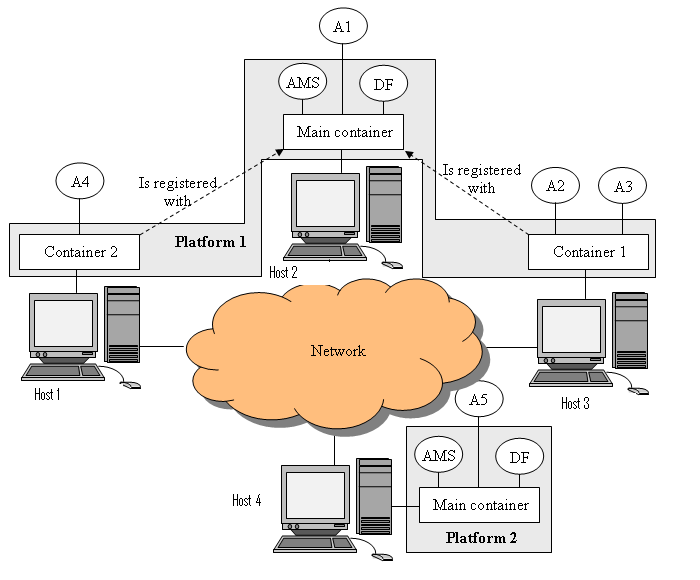
\includegraphics[width=\textwidth]{fig/jadeArchitecture}
	 	\caption{JADE Architechture}
	 	\label{fig:JADEarchitechture}
	 	%Figure found at http://jade.tilab.com/doc/tutorials/JADEAdmin/jadeArchitecture.html
	 	\todo[inline]{Consider remaking this figure so we don't have to cite it}
 \end{figure}

Details of our implementation can be found in Section \ref{sec:architecture}.

\section{Homomorphic Encryption}\label{sec:homomorphic_encryption}
Homomorphic encryption is an encryption scheme which allows computations to be carried out on ciphertext, meaning plaintext that has been encrypted using an algorithm and a public key. The result of the computations is also encrypted, and can be deciphered back to plaintext using a private key. This has long been considered crypthography's holy grail \citep{Micciancio2011HomoEnc}, as this would allowing operating on encrypted text without knowing the decryption key. For example, given ciphertexts $C_1=Enc(Data1)$ and $C_2=Enc(Data2)$, an additively homomorphic encryption scheme would allow to combine $C_1$ and $C_2$ to obtain $Enc_K(Data1+Data2)$. More concretely this means that if you encrypt your data using such an encryption scheme, you can transfer your data to an untrusted server which can perform some arbitrary computations on that data without being able to decrypt the data itself.

Up until recently, all published homomorphic encryption schemes only supported one basic operation, most commonly addition. These schemes could only be called partially homomorphic, as they did not provide any extensive functionality. The notion of a  fully homomorphic encryption schemes was first proposed by \cite{rivest1978data}, but it wasn't realized until 2009 when Craig Gentry published a doctoral thesis where he proved that he had constructed a fully homomorphic scheme\cite{gentry2009FHEpaper}. Gentry's solution was based on "ideal lattices" as well as a method to double-encrypt the data in such a way that the errors could be handled "behind the scenes". By periodically unlocking the inner layer of encryption underneath an outer layer of scrambling, the computer could hide and recover from errors without ever analyzing the secret data. 


The downside of Gentry's two-layered approach is that it requires a massive computational effort. Bruce Schneier, a leading American cryptographer, pointed out "Gentry estimates that performing a Google search with encrypted keywords -- a perfectly reasonable simple application of this algorithm -- would increase the amount of computing time by about a trillion. Moore's law calculates that it would be 40 years before that homomorphic search would be as efficient as a search today, and I think he's being optimistic with even this most simple of examples\citep{schneier2009blog}." 


%\section{Resource consumption}
%\todo{Give analysis of time and space complexities and how much this taxes a device.}


\cleardoublepage
